
%


\section{Tools}\label{sec:tools}

\renewcommand{\kapitelautor}{Autor: Nils} % todo: replace

\subsection{Jira}\label{subsec:jira}
%
Jira ist ein Softwaretool welches im Fall von .Forty-Five als Scrum Planungssoftware verwendet wurde.
Es besteht aus einem Product Backlog, in dem alle Tasks in Form von Epics und Userstories abgelegt sind.
Dieser wird vom Scrum Master und Product Owner gepflegt, um Fortschritt zu überwachen und den Mitarbeitern genaue Vorgaben über ihre Aufgaben zu liefern.
Diese Aufgaben werden in Form von Epics definiert und in einzelne User Stories aufgeteilt.
Weitergehend wird die Aufgabe einem Teammitglied zugeordnet und die Größe der einzelnen Arbeitspakete mittels Planningpoker geschätzt, um den Aufwand einzuschätzen.
Planning Poker ist ein Kartenspiel, das zur Aufwandseinschätzung dient. Die Teammitglieder haben Karten mit Fibonacci Zahlen und jeder Teammitglied schätzt die Größe einer User Story.


%\begin{figure}[H]
%    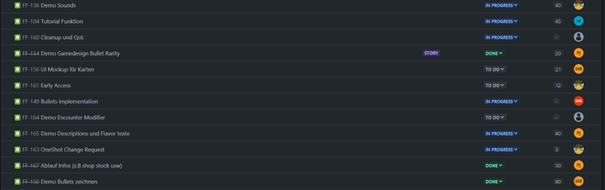
\includegraphics[width=\textwidth]{Backlog.png}
%    \caption{Backlog}
%\end{figure}

\subsection{Trello}\label{subsec:Trello}
%
Die Software Trello ist ein Projektmanagement Tool im Kanban Stil. Es stellt ein Board dar, welches mit Karten befüllt wird.
Das Board ist in Spalten unterteilt, welche zur Kategorisierung oder zur Fortschrittseinteilung genutzt werden können.
Außerdem können Personen zu den Tasks zugewiesen werden, Aufwandseinschätzungen zugeordnet und Zeit getrackt werden.
Es ermöglicht eine einfache Übersicht durch die einfache simple Darstellung
%\begin{figure}[H]
%    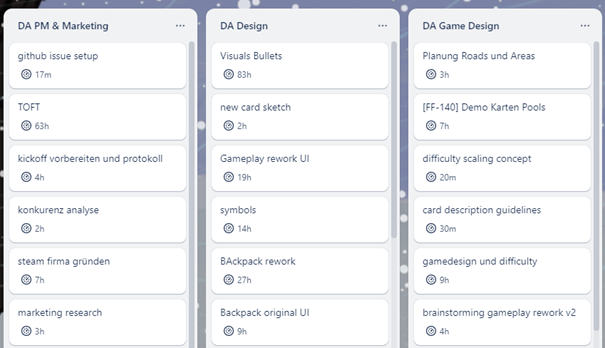
\includegraphics[width=\textwidth]{Trello_log.png}
%    \caption{Trello}
%\end{figure}
%
\subsection{Discord}\label{subsec:Discord}
Discord ist eine Kommunikationsplattform, die primär zur internen Kommunikation verwendet wurde, da sie viele Möglichkeiten der Kommunikation kombiniert.
Es sind sogenannte Voice Channels vorhanden, welche es den Teammitgliedern erlauben zusammen zu arbeiten und sich während der Arbeit auszutauschen.
Es gibt Textkanäle die zum Versenden von Nachrichten, Informationen oder Dateien ermöglichen. Außerdem dient es als soziale Plattform um sich eine Community aufzubauen.

%\begin{figure}[H] 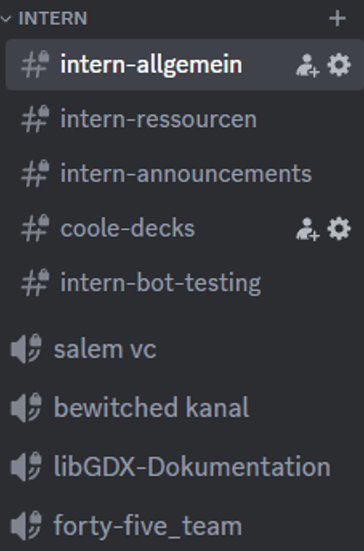
\includegraphics{Discord.png}\caption{Discord}
%\end{figure}
%

% resets author
\renewcommand{\kapitelautor}{}
